\section{Results}
\label{sec:results}

\subsection*{Replacement damage concentrates at identifiable steps}

Task-level pass rates conflate two questions that must be separated before model allocation can be reasoned about: whether an agent can solve a task, and \emph{where} in its execution it genuinely requires frontier capability. We therefore froze complete trajectories produced by a frontier model on scientific-computing tasks and re-executed them from individual steps, replacing only the policy at that step while holding context, tool state, and remaining budget fixed \begin{figure}[tb]
\centering
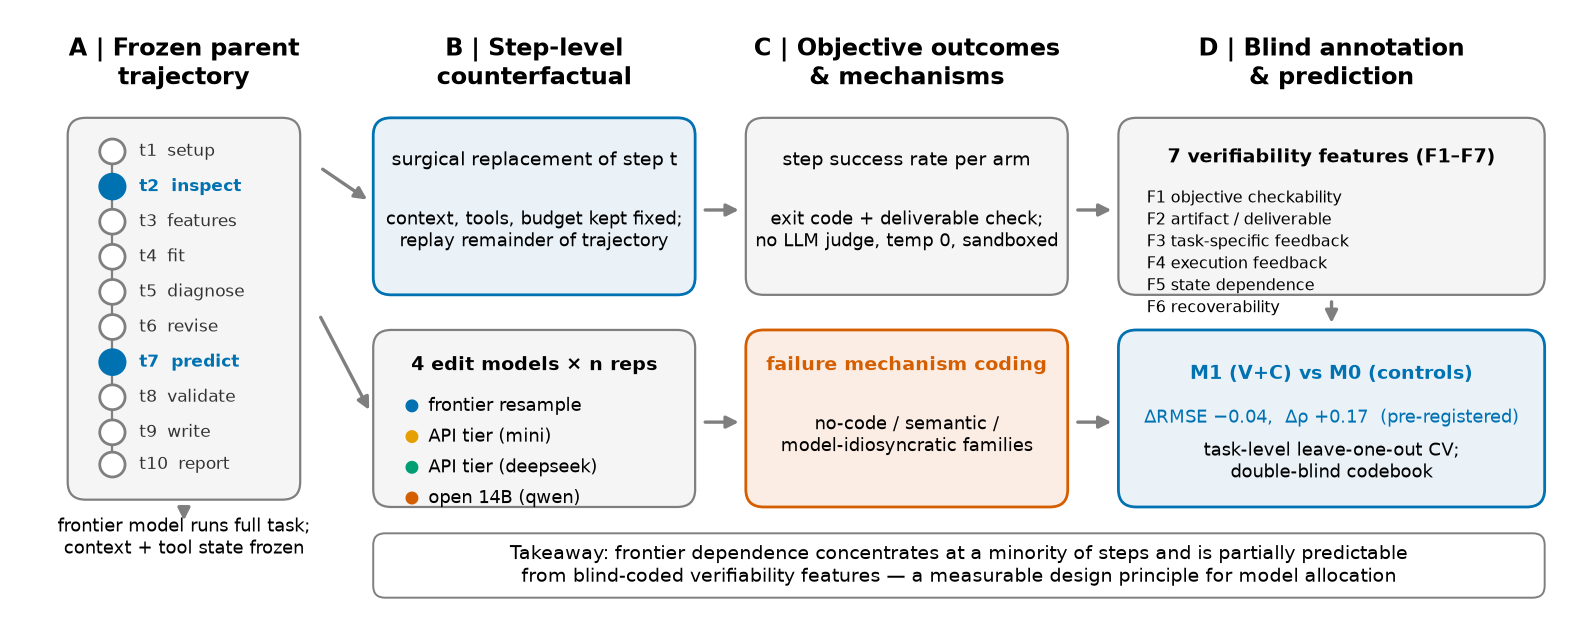
\includegraphics[width=\linewidth]{figures/fig1_framework.png}
\caption{Overview of the step-level counterfactual replacement framework. A frozen frontier parent trajectory (A) is probed at individual steps (B): the selected step is regenerated by one of four replacement arms under identical context, tool state and remaining budget, while the frontier policy resumes all subsequent steps (C). Outcomes are adjudicated objectively, replacement-step transcripts are coded into error families, and signal/control points feed the blind annotation stage (D), in which two annotators score seven verifiability features from frozen reading materials before any outcome is examined.}
\label{fig:framework}
\end{figure}

(Fig.~\ref{fig:framework}; Methods). Across 705 in-point runs spanning 38 step instances, four replacement arms --- frontier resampling and three cheaper edit models (two API-tier models, mini and DeepSeek, and an open-weights Qwen3-14B) --- we asked a simple question at each step: does the cheaper model, given exactly the same situation, reproduce what the frontier model did?

The answer varies far more across steps than across tasks. Difference-in-differences against matched control steps isolates the step-specific component of replacement damage: relative to their behaviour on ordinary steps, cheaper models lose 0.21 (mini), 0.25 (DeepSeek) and 0.71 (Qwen) success probability at the six identified signal steps (pooled controls; the ordering is preserved under a common-control-set calibration: -0.24, -0.27, -0.63). That the largest open-weights model in our sweep suffers the most step-specific damage is not a paradox of capability but a signature of behaviour: error-family coding of the replacement-step transcripts shows that Qwen's signal-step failures are dominated by a model-idiosyncratic error family (25 of 52 runs) that neither API model produces at scale, whereas the API models fail predominantly by emitting no code at all (protocol lapses) and the frontier resamples essentially never err at the step level (Fig.~\ref{fig:mechanisms}b). Failure at a step is thus not a graded attenuation of frontier behaviour but a discrete, model-characteristic event --- an observation that motivates treating steps, not tasks, as the unit of analysis.

\begin{figure}[tb]
\centering
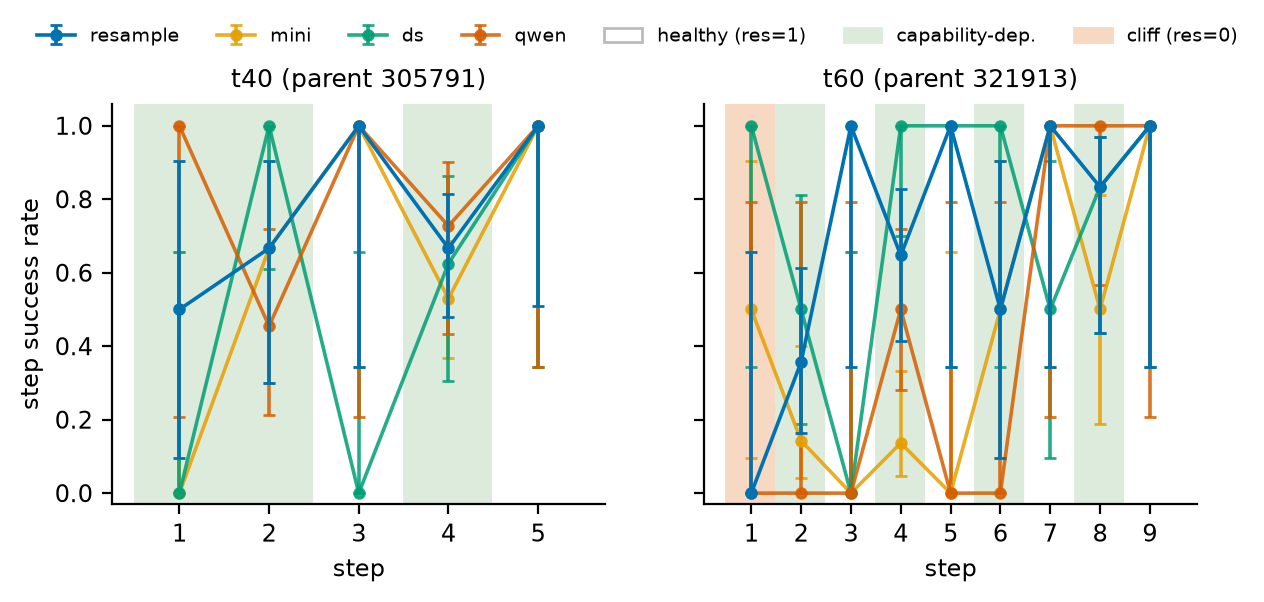
\includegraphics[width=\linewidth]{figures/fig2_scan_profile.png}
\caption{Full-step replacement profiles for parent trajectories t40 (a) and t60 (b). Each point shows the success rate of one (step, arm) cell with Wilson 95\% intervals; the frontier-resample baseline defines three step classes (healthy, capability-dependent, cliff) marked by the side band.}
\label{fig:scan}
\end{figure}

\subsection*{Full-step profiles separate healthy, capability-dependent and cliff steps}

Aggregating over single signal points risks missing structure that only a dense scan can reveal. We therefore swept every step of two representative parent trajectories (t40, five pre-deliverable steps; t60, nine steps) across all four arms under the same counterfactual protocol, yielding 193 sandbox-valid runs and a complete per-step, per-arm success-rate surface (Fig.~\ref{fig:scan}). Three step classes emerge from the resample baseline alone. \emph{Healthy} steps (resample success 1.0) tolerate every replacement arm within confidence limits. \emph{Capability-dependent} steps show graded degradation that tracks model capacity. \emph{Cliff} steps --- where resampling itself fails --- behave discontinuously: at t60s2, t60s3 and t60s6, no arm recovers more than a fraction of frontier performance, and at the single-step replacement level mini reaches only 0.14--0.50.

Two cautions temper this surface. First, per-cell replication remains small enough that no individual step-arm contrast survives BH-FDR correction at q < 0.10 across the 42 tests of the scan snapshot --- the informative content of the scan is the \emph{profile shape} (concentration and classification), not any single cell. Second, the cliff class is defined by the frontier baseline's own failure, so it identifies steps whose difficulty is intrinsic rather than model-relative. Both cautions are addressed by the aggregation and intervention analyses below, which is why we position the scan as descriptive anatomy rather than confirmatory evidence.

\begin{figure}[tb]
\centering
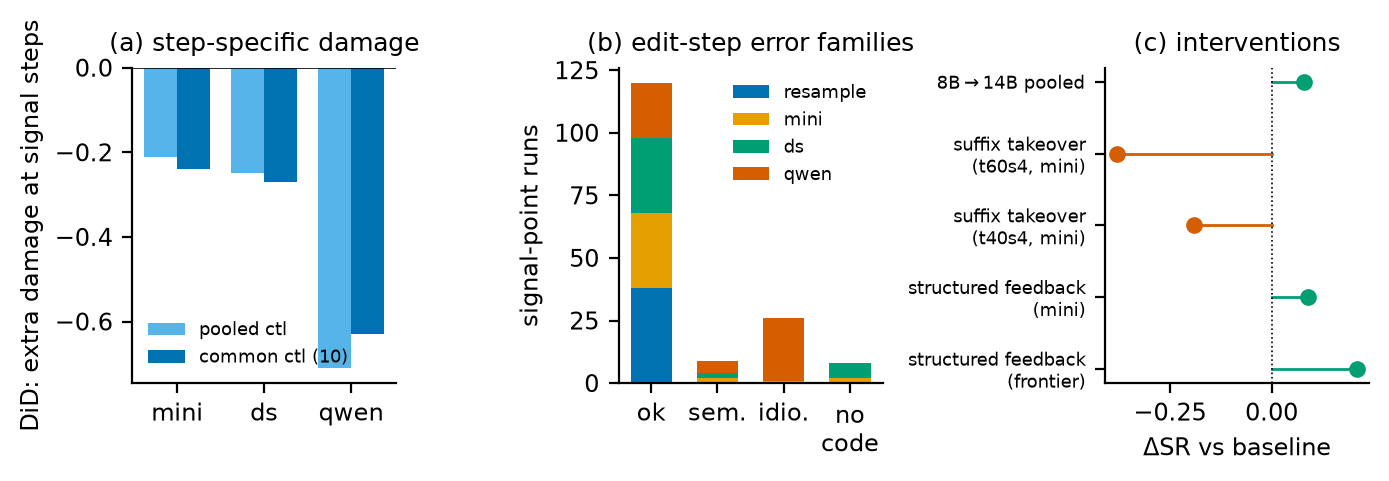
\includegraphics[width=\linewidth]{figures/fig3_mechanisms.png}
\caption{Mechanistic evidence. (a) Step-specific replacement damage (difference-in-differences against matched controls) for the three edit arms under pooled and common-control calibrations. (b) Error-family composition of replacement-step failures at the six signal points: protocol lapses dominate for the API arms, a model-idiosyncratic family for the open-weights arm. (c) Intervention effects: structured feedback repairs while suffix takeover amplifies damage.}
\label{fig:mechanisms}
\end{figure}

\subsection*{Structured feedback repairs; naive splicing amplifies}

If step-level failures are discrete events rather than graded attenuation, they should respond to targeted intervention --- and respond differently to interventions that respect versus violate step boundaries. We tested three interventions at the signal steps (Fig.~\ref{fig:mechanisms}c). First, structured feedback: when a replacement step fails, re-prompting the edit model with a structured diagnosis of the failure (error class, expected output contract, failing assertion) raises frontier-step success from 0.54 under bare retry to 0.75, and mini's from 0.33 to 0.42, while consuming fewer retry rounds (1 of 12 versus 3 of 13). The repair is partial rather than complete, consistent with a residual component of genuine capability gap that feedback cannot substitute. Second, suffix takeover --- splicing the cheaper model's edit into the frontier trajectory and letting the frontier model continue from there --- \emph{amplifies} damage rather than containing it: mini's success falls from 0.33 (single-step replacement) to 0.14 at t40s4 and from 0.38 to 0.00 at t60s4. The information a frontier model needs to recover from a foreign edit is evidently not recoverable from the edit's surface form; step boundaries are not clean interfaces for heterogeneous policies. Third, scale alone does not dissolve the failure: doubling Qwen from 8B to 14B leaves pooled signal-point success statistically indistinguishable (0.37 versus 0.45, Fisher p = 0.61), with two signal points repaired, two persisting and two newly failing --- the idiosyncratic error family migrates rather than vanishes.

A final control concerns the experimental machinery itself: runs that exhaust the step budget are not silently counted as failures but re-executed under a protocol retry, and their final success rate (4 of 8) matches matched controls (4 of 8), confirming that budget exhaustion is an artifact of the observation window rather than a property of the replaced steps.

\begin{figure}[tb]
\centering
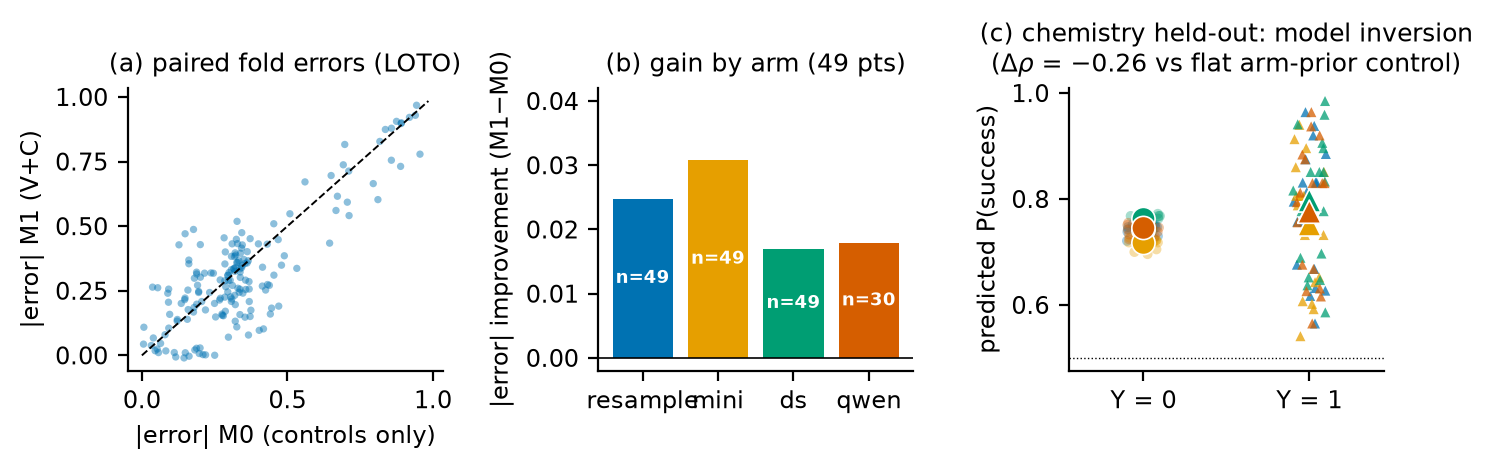
\includegraphics[width=\linewidth]{figures/fig4_prediction.png}
\caption{Blind-coded verifiability features predict step-level replaceability in distribution, and invert out of it. (a) Leave-one-task-out paired absolute errors over the enlarged 49-point set: the feature model (M1) improves on the arm-prior control (M0) for most observations ($\Delta$$\rho$ +0.13, paired permutation p = 0.001). (b) Per-arm improvement attributable to features; all four arms benefit. (c) On the 18-point Computational Chemistry held-out set, both models produce near-identical predictions for failed and succeeded outcomes --- the feature model's outcome mapping reverses across domains, ranking success worse than the flat arm-prior control ($\Delta$$\rho$ $-0.26$).}
\label{fig:prediction}
\end{figure}

\subsection*{Blind-coded verifiability features predict step-level replaceability}

The preceding results establish \emph{that} frontier dependence concentrates and \emph{how} it fails; they do not yet say whether one could have predicted where, from properties of the step alone. We posed this as a pre-registered prediction problem. Two annotators --- one of them an AI assistant with declared contamination limits, one the project lead, both blind to all per-point replacement outcomes --- independently coded seven verifiability features for each of the 38 step instances from frozen reading materials (task instruction, step code, truncated observation, step transcript) generated by a script with machine checks against leakage. Inter-annotator agreement passed for the two features with mechanical definitions (weighted $\kappa$ = 0.83 for artifact production, 1.00 for step type) and fell below 0.6 for the five judgement-laden features, triggering a pre-registered two-round clarification and adjudication protocol over a {0, 0.5, 1, 1.5, 2} value grid; the merged 38 $\times$ 7 matrix (128 cells by agreement, 81 by one-level averaging, 17 by adjudication, 2 by annotator-A default) was frozen with a timestamp before any per-point outcome was examined.

Under task-level leave-one-out cross-validation with fixed regularisation (no tuning leakage), a ridge model adding the six feature scores to step position, remaining budget, stratum, role and arm identity reduces prediction error of per-arm success rate by 0.036 RMSE and raises Spearman correlation from 0.30 to 0.47 --- meeting both pre-registered criteria ($\Delta$RMSE $\leq$ 0, $\Delta$$\rho$ $\geq$ 0.1) for the hypothesis that verifiability carries independent predictive signal (Fig.~\ref{fig:prediction}). A gradient-boosting sensitivity check reproduces the direction. The gain is not uniform: it concentrates on the API arms and is driven largely by the distinction between exploratory steps --- which lack an objective correctness standard and are therefore unusually safe to delegate to cheaper models --- and deliverable-producing steps, which are not. For the open-weights arm, whose failure signature is nearly collinear with its identity, features add nothing beyond the arm indicator, an honest boundary on what verifiability profiling can and cannot do. With 38 step instances the result is directional rather than definitive, and we report it with the pre-registered power caveat attached; the F2 artifact measure is an operational proxy for deliverable production, not a claim that agents possess semantic verifiers at runtime.

To probe external validity we re-fitted both models on the full annotated set and asked them to predict the seven scan step instances that lie outside the 38-point selection yet carry complete four-arm outcomes (28 observations), first with all tasks in training and then with the two scan tasks removed entirely. The gain does not survive this move: at the instance level the feature model's rank correlation falls from +0.47 (in-protocol) to $-0.20$ against matched controls, and at the task level to $-0.27$, with a permutation test placing the held-out estimate inside the null range (p = 0.16 for the observed negative value at n = 28). Three mechanisms plausibly contribute: five of the seven held-out instances are exploration or inspection steps, a regime in which training saw little between-arm variance to discriminate; early-step outcomes in the scan trajectories are dominated by downstream cliff variance rather than by the replaceability of the step itself; and the feature model's predictions collapse to a narrow mean-plus-arm-prior band on out-of-distribution points. We therefore report the pre-registered H2 result as valid within the annotated point distribution under the frozen sampling protocol, and treat out-of-distribution prediction of replaceability as an open problem that the measured ground truth produced by this protocol is positioned to solve, since each newly annotated point extends exactly the regime in which the features demonstrably work.

The same protocol executed end-to-end on a fully unseen domain sharpens this boundary into a prospective result. Two Computational Chemistry tasks --- a domain with zero representation among the 14 training tasks --- were carried from parent run through blind annotation to a complete 46-run replacement grid (6 points $\times$ 4 arms, Methods). Their ground truth is instructive in itself: every arm succeeded at every point of the regression task, including at a step that had failed in its own parent trajectory, while the classification task's deliverable step survived only under deepseek edits. Against this target, the feature model shows no significant advantage under any of three training configurations (38, 30, or 45 points): the rank-correlation difference spans $-0.02$ to $+0.19$ with permutation p $\geq$ 0.28 in every variant, and RMSE is never improved (all $\Delta$RMSE $\geq$ 0). The failure is mechanistic rather than noisy: the feature model imports the training domain's prior that late deliverable-producing steps with inherited context tend to fail, and assigns the chemistry deliverable steps predictions of 0.26--0.31 where all four arms in fact succeeded (p = 1.00) --- the feature--outcome mapping for this stratum reverses across domains, while the control model's flat arm-prior predictions are merely uninformative.

Two pre-registered extensions settle the two open questions this pattern raises. First, does the in-distribution result strengthen at the pre-registered sample size? Eleven new points from six in-distribution parents (Methods, scale-up) fold into the leave-one-task-out analysis: the feature model retains its advantage with both pre-registered criteria met ($\Delta$RMSE $-0.016$, $\Delta$$\rho$ +0.13, against +0.17 on the original 38 points), and a paired permutation test that swaps the two models' predictions within each point now makes the gain formally significant ($\Delta$$\rho$ +0.129, two-sided p = 0.001 over 20,000 permutations, n = 177 observations), so the H2 result is a replicated in-distribution regularity rather than a small-sample artifact, and the annotated-point total (74) retires the sample-size caveat. Second, was the cross-domain null merely underpowered? Twelve further Chemistry points from two new parents triple the held-out set to 18 points and 72 observations. The answer is decisive in the negative direction: under every training configuration the feature model is \emph{worse} than the arm-prior control in rank correlation ($\Delta$$\rho$ between $-0.18$ and $-0.27$; paired permutation p = 0.07 in the primary 49-point configuration and p = 0.11--0.17 across variants, 20,000 permutations each) and worse in RMSE in all variants, and the new ground truth contains exactly the cells the feature model most misreads --- a deliverable step that every arm fails on a 12-step trajectory, and a modelling step where deepseek and the frontier baseline collapse while the open-weights replacement succeeds. Verifiability profiling therefore measures real structure, but the structure it measures is local: the reliable path to extending it is one measured domain at a time, at roughly seven dollars per domain-cycle, not a leap of faith about what verifiability means elsewhere.
